\documentclass[10pt]{article}
\usepackage[margin=0.75in]{geometry}
\usepackage{graphicx}
\usepackage[T1]{fontenc}
\usepackage{lmodern}
\usepackage{xcolor}
\usepackage{hyperref}
\hypersetup{colorlinks=true,urlcolor=blue}
\title{RM Kummer FFT rounding guard correction}
\author{Implementation validation note}
\date{25 October 2026}
\begin{document}
\maketitle
\noindent\textbf{Scope.} Source snapshot \texttt{af671797}. No archived survey record or performance value is changed.

\medskip
\noindent\textbf{Observed discrepancy.} The frozen survey README says the FFT point counter raises when its output is more than $10^{-3}$ from an integer. The previous code required that absolute condition \emph{and} an additional relative condition. The synthetic value $S=6000.003$ has residual $0.003$ but passes the old guard because $0.003 < 10^{-6}|S|$. NaN and infinity also bypassed those comparisons. These are guard counterexamples, not observations from the archived survey.

\medskip
\noindent\textbf{Repair.} Reject nonfinite output, then raise whenever $\max|S-\mathrm{round}(S)|>10^{-3}$. The targeted regression injects all three counterexamples; the existing small-prime FFT versus brute-force order test remains a separate control. Targeted result: four passed, eleven deselected. The full RM/Q-curve test module passed fifteen of fifteen.

\begin{center}
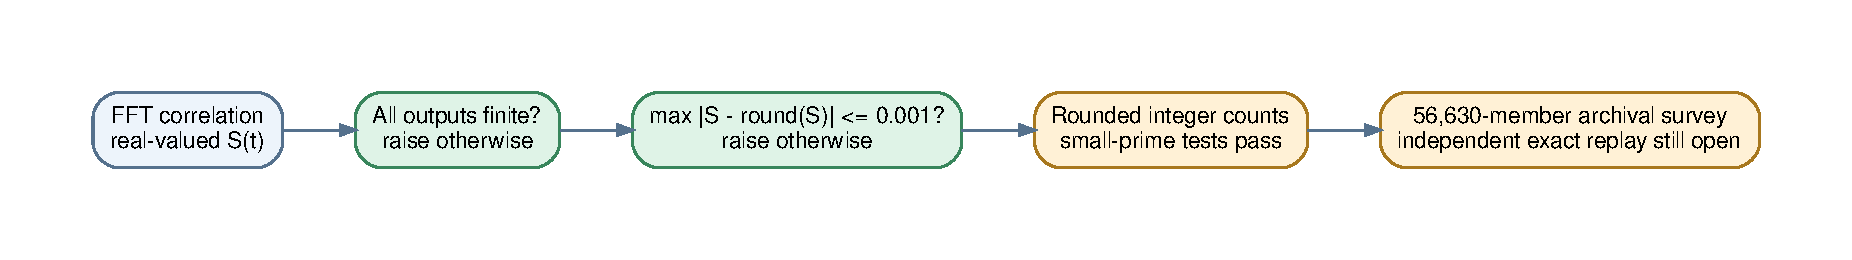
\includegraphics[width=\linewidth]{guard-diagram.pdf}
\end{center}

\noindent\textbf{Boundary.} This check does not certify the true integer character sum for each archived member. The 56,630-member RM survey, 5,628 split cases and 859 recorded hits have a separate summary-arithmetic check and 12 reported PARI spot checks, but no independent exact member-by-member replay or original loaded-source custody. No canonical measured graph changes.

\medskip
\noindent An open problem record tracks the exact-census and source-custody obligations. Future generated survey prose now labels the FFT counts as rounded results and states the validation limit.

\medskip
\noindent\textbf{Reproduction.} See \texttt{REPORT.md}, \texttt{guard.dot}, the changed \texttt{rmkummer.py}, and \texttt{tests/test\_endosweep\_rm\_qcurves.py} in this branch. The diagram shows the corrected guard and the remaining archival-validation boundary.
\end{document}
